% -*- mode: LaTeX; coding: utf-8; -*-

\chapter{Analyysi}

Tässä luvussa käydään vaiheittain läpi yhden valitun palvelun analysointi sekä esitetään perustelut, joiden pohjalta tehtyihin ratkaisuihin on päädytty. 
Luvussa myös esitellään analysoinnista saatuja tuloksia sekä pohditaan näihin johtaneita syitä. Lopuksi vielä esitetään jatkotutkimuksen kannalta 
tärkeitä kehitysideoita, joita syntyi tutkimuksen aikana. 
 
\section{Tutkimuksen toteutus}

Saamamme materiaali koostui neljästä eri Web-palvelusta, joista analyysiin valitsimme yhden. Muista palveluista saadut lokitiedostot käsiteltiin
myös valmiiksi, mutta koska lokitietoja oli määrällisesti niin paljon, päädyimme tarkastelemaan tarkemmin vain yhtä. Valitsemastamme palvelusta
analysoimme myös vain viikon mittaisen jakson. Tähän ratkaisuun päädyttiin sen takia, että analysoitavaa dataa oli kerätty noin puolen vuoden ajalta,
joten jo yhden palvelun osalta koko datan läpikäymiseen olisi mennyt kohtuuttomasti aikaa. Käytetyn menetelmän rajoitukset, jotka on kerrottu luvussa \ref{sec:matlab},
asettivat myös käytännön rajoituksia analysoitavien tiedostojen määrälle. Tämän kokoinen otanta oli kuitenkin riittävän suuri esikäsittelijän toimivuuden
testaamiseen, jonka lisäksi käytettyjen menetelmien sopivuutta käytössä olleen materiaalin analysoimiseen voitiin arvioida. 

Esikäsittelyvaiheessa HTTP-kyselyt jaetaan palvelun resurssien mukaan
omiin tiedostoihin, joissa ne ovat CSV-formaatissa kuvan \ref{csv882}
mukaisesti.  Resursseihin kohdistuvien kyselyiden lukumäärä vaihtelee
suuresti sen mukaan, kuinka käytetty mikäkin resurssi on. Web-sivun
ollessa kyseessä lukumäärä vastaa sivun käyntimäärää. Mikäli resurssia
käytetään esimerkiksi muun sivun osana, kuten tyylitiedostojen ja
kuvien tapauksessa, tämä kasvattaa merkittävästi kyselyiden lukumäärää
verrattuna tavanomaiseen Web-sivuun.

Analyysissä käyttämämme viikon pituinen jakso sisälsi yhteensä 913 eri
resurssia ja näihin kohdistuvat kyselymäärät vaihtelivat muutamasta
kappaleesta aina kymmeniin tuhansiin. Koska Web-palveluihin kohdistuvat 
tietoturvahyökkäyksissä hyödynnetään erityisesti HTTP-kyselyn parametriosan 
käsittelyn haavoittuvaisuuksia, keskityimme vain sellaisiin palveluihin, joissa 
esiintyi vaihteleva kirjo parametreja. Tämä rajaus tehtiin suodattamalla pois sellaiset
resurssit, joihin kohdistui alle sata kyselyä ja joiden
GET-parametreista muodostettujen erilaisten n-grammien määrä oli alle
kymmenen. Suodatuksen jälkeen analysoitavaksi jäi 36
resurssia. Suodatus suoritettiin esikäsittelyn jälkeen ja
suodatusrajat on säädettävissä PhasefulSplitterin tiedostosta
\texttt{src/InterestingParameters.hs}.

Käytetyimmissä resursseissa HTTP-kyselyitä oli kymmeniä tuhansia,
joten jokaisesta resurssista ei pystytty suoraan tekemään
diffuusiokuvausta johtuen menetelmän rajoituksista. Ongelma
ratkaistiin valitsemalla satunnaisotannalla ilman takaisinpanoa 2~000
HTTP-kyselyä niistä resursseista, joissa oli kyselyitä yli tämän
määrän. Näin ollen jokaisesta resurssista muodostettiin lopulta
tiedosto, jossa oli enintään 2~000 HTTP-kyselyä.

\begin{figure}[hb]
\centering
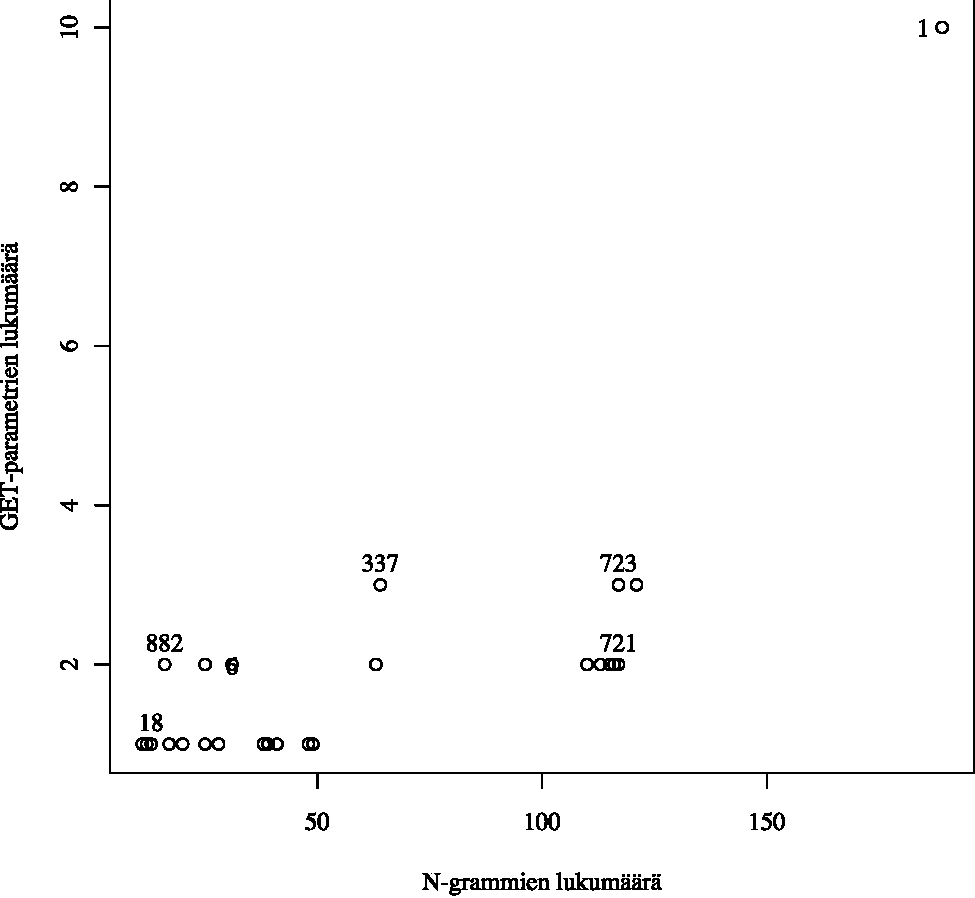
\includegraphics[width=13cm]{pics/service_resources.pdf}
\caption{Palvelun resurssien ominaisuudet.}
\label{service_resources}
\end{figure}

Analysoitavan palvelun eri resurssit on esitetty kuvassa
\ref{service_resources}. Kuvassa vaaka-\-akselina on käytetty
N-grammien lukumäärää ja pystyakselina GET-parametrien
lukumäärää. Resursseista valitsimme kuusi tarkempaan tarkasteluun ja
ne on merkitty kuvaajaan niiden resurssinumerolla.  Resurssit pyrimme
valitsemaan siten, että jokaisesta ryppäästä olisi yksi valittuna.

Palvelun jokaisesta resurssista muodostettiin aluksi diffuusiokuvaus
käyttäen edellä kuvatulla tavalla suodatettua aineistoa.
Analysoimalla saatua diffuusiokuvausta voitiin määrittää ne pisteet,
jotka oli luokiteltu poikkeaviksi siinä joukossa, jossa kyseisiä
pisteitä oli verrattu. 

Seuraavaksi lasketuista diffuusiokuvauksista muodostettiin
diffuusiokartta käyttäen toista ja kolmatta ominaisvektoria. Koska
suuri määrä pisteitä sijoittui täsmälleen samoihin koordinaatteihin,
kartan luettavuuden parantamiseksi sirontakuvion pisteitä
``täristettiin''. Täristäminen suoritettiin lisäämällä
ominaisvektorien arvoihin normaalijakaumasta satunnaisesti poimittu
arvo. Normaalijakauman keskihajontana käytettiin yhtä prosenttia
akselin leveydestä. Kuvassa \ref{diffuusio_1} nähdään edellä kuvatulla
tavalla muodostettu diffuusiokartta resurssista 1. Kuvaajasta voidaan
havaita, että muutamaa poikkeusta lukuun ottamatta pisteet sijoittuivat
hyvin lähelle toisia.

Diffuusiokartta ei ole sellaisenaan kovinkaan havainnollinen, joten
jokaiselle pisteelle laskettiin vielä poikkeavuusluku. Se muodostettiin
summaamalla euklidinen etäisyys lähimpään kolmeen pisteeseen
diffuusiokuvauksen toisen, kolmannen ja neljännen ominaisvektorin
muodostamassa diffuusioavaruudessa. Tämän etäisyystiedon avulla voitiin piste
luokitella poikkeavuudeksi sekä piirtää poikkeavuuskartta.

Kuvassa \ref{service_1} on resurssista 1 muodostettu poikkeavuuskartta. Kuvaajassa vaaka-akselille on sijoitettu resurssille kohdistuneet HTTP-kyselyt
ja pystyakselin mittana on poikkeavuus. Tässä pystyakseli ilmaisee sen kuinka poikkeava kukin piste on vertailujoukon sisällä. Jokaiselle kuvaajalle
on vielä määritetty keskihajonta ja raja-arvo, jonka ylittäneet pisteet merkitään poikkeaviksi. Tämä raja-arvo vaihtelee tapauskohtaisesti ja sen
arvo on kolme kertaa keskihajonta. Keskihajonta on merkitty kuvaajaan katkoviivalla ja raja-arvo yhtenäisellä viivalla. Esimerkiksi resurssin 1 
poikkeavuuskartassa \ref{service_1} on nähtävissä viisi poikkeavuudeksi merkittyä pistettä.

Jokainen diffuusiokartan luomiseen käytetty piste pystytään
palauttamaan siihen HTTP-kyselyyn, josta se on
muodostettu. Esitetyissä kuvaajissa palauttamiseen tarvittavat tiedot
on merkitty niihin pisteisiin, jotka ylittävät raja-arvon. Otetaan
esimerkiksi kuvaajan \ref{service_18} ainoaksi merkitty poikkeama,
jolla on arvot ovat 7,3 ja 14594. Näistä ensimmäinen arvo ilmoittaa
sen tiedoston järjestysnumeron, josta kyseinen HTTP-kysely
löytyy. Seuraava luku puolestaan kertoo sen palvelimen
järjestysnumeron, johon kysely on ohjattu. Näiden kahden luvun avulla
voidaan yksilöidä tietty lokitiedosto. Viimeisin luku sisältää
rivinumeron kyseisen lokitiedoston sisällä.

\section{Tulokset}

Analysoitavassa materiaalissa resurssilla 1 (kuva \ref{service_1}) oli
viisi HTTP-kyselyä, jotka merkittiin poikkeaviksi. Tutkimalla
diffuusiokuvauksen luomiseen käytettyä lokia, ja palauttamalla
HTTP-kyselyt alkuperäiseen muotoon, pystyimme paikallistamaan nämä
kyselyt ja vertaamaan niitä lokin muihin kyselyihin. Resurssin 1
tapauksessa neljä poikkeavaksi merkittyä kyselyä sisälsivät sellaisen
GET-parametrin, jota ei esiintynyt muissa kyselyissä. Parametri
vaikutti olevan jonkinlainen tunniste, jolla käyttäjä oli mahdollista
yksilöidä. Jäljelle jääneessä kyselyssä esiintyi useita eri
GET-parametreja, joita kyseinen resurssi ei käsittele. Tämä on
saattanut yksinkertaisesti johtua siitä, että käyttäjä on kopioinut
Web-sivun osoitteen selaimeensa virheellisesti.

Kuvassa \ref{service_18} on nähtävillä resurssin 8 poikkeavuuskartta. Kyseisessä otannassa oli mukana 181 pistettä ja näistä kaksi todettiin poikkeavaksi.
Resurssi 8 tarjosi vain staattista sisältöä, joten GET-parametrin jälkeistä kyselyosuutta ei HTTP-kyselyissä pitänyt olla. Yhdessä poikkeavassa kyselyssä oli
GET-parametrin resurssipolun jälkeen kuitenkin kysymysmerkki ja tämän perässä oli pyynnön tehneen alustan verkko-osoite. Tämän poikkeavan kyselyn tunnistaminen
oli helppoa, sillä se oli ainoa kysely, jolle n-gram -analyysi tuotti
nollasta poikkeavia arvoja. Resurssille tehty kysely oli selkeästi virheellinen, sillä merkitty verkko-osoite 
oli privaattiverkon osoite. Kyselyssä käytetty alusta oli myös ainoa laatuaan. Toinen poikkeavaksi merkitty kysely oli myös helppo tunnistaa, koska siinä 
käytetty metodi oli muista poiketen HEAD. Tarkempi analyysi osoitti, että kysely oli peräisin automaattisesta robotista, joka indeksoi Web-sivuja. 

Resurssissa 337 (kuva \ref{service_337}) poikkeavuuksia havaittiin kuusi kappaletta. Näistä neljässä oli GET-parametrina samanlainen tunnistetieto
kuin resurssin 1 kolmessa havaitussa poikkeavuudessa. Yksi poikkeavuus taas oli saman käyttäjän aiheuttama kuin resurssilla 8, sillä kysely tuli samasta
verkko-osoitteesta ja näiden välillä ei ollut kulunut kuin muutama
minuutti. Käytetty alusta oli myös ainoa laatuaan ja kyselyn yhtenä parametrina oli 
sama verkko-osoite. Onkin hyvin todennäköistä, että kyselyt
kohdistuivat väärään palveluun, koska kyselyiden oikeassa muodostuksessa ilmeni
virheitä. Viimeisessä poikkeavassa kyselyssä oli sitten muista eroava määrä avain-arvo pareja.

Molempien kuvien \ref{service_721} ja \ref{service_723} poikkeavuudet yhtä lukuunottamatta
aiheutuivat GET-parametrista, jota ei esiintynyt muissa
kyselyissä. Ylimääräisen parametrin nimi oli sama kuin resurssissa 1,
ja niistä jokainen tuli samasta IP-osoitteesta. Parametrin arvo
kuitenkin vaihteli kyselystä riippuen. Tämä viittaa siihen, että
kyselyt olivat tulleet välityspalvelimen kautta, joka jostakin syystä
lisää kyseisen tunnistetiedon. Tämän takia sen kautta tulevat pyynnöt
näyttävät erilaiselta. Palvelin kuitenkin oli osannut käsitellä nämä
kyselyt normaalisti, sillä HTTP-\-vastauskoodi näiden kyselyiden
osalta oli 200. Viimeinen poikkeavuus oli sitten samanlainen kuin kuvassa \ref{service_18} eli kyselyssä oli pyynnön tehneen alustan verkko-osoite.

Viimeisen analysoidun resurssin (kuva \ref{service_882}) kahdesta
havaitusta poikkeavuudesta yksi johtui samanlaisesta tunnistetiedosta,
joka esiintyi myös aikaisemmissa kuvissa. Toinen poikkeavuus sisälsi 
myös ylimääräisen GET-parametrin, mutta aiemmista tapauksista poiketen 
tämä oli perinteisempi parametri, jota ei kuitenkaan olisi pitänyt
välittää palvelimelle. Tästä huolimatta palvelin oli osannut käsitellä
kyselyn. 


\begin{figure}[p]
\centering
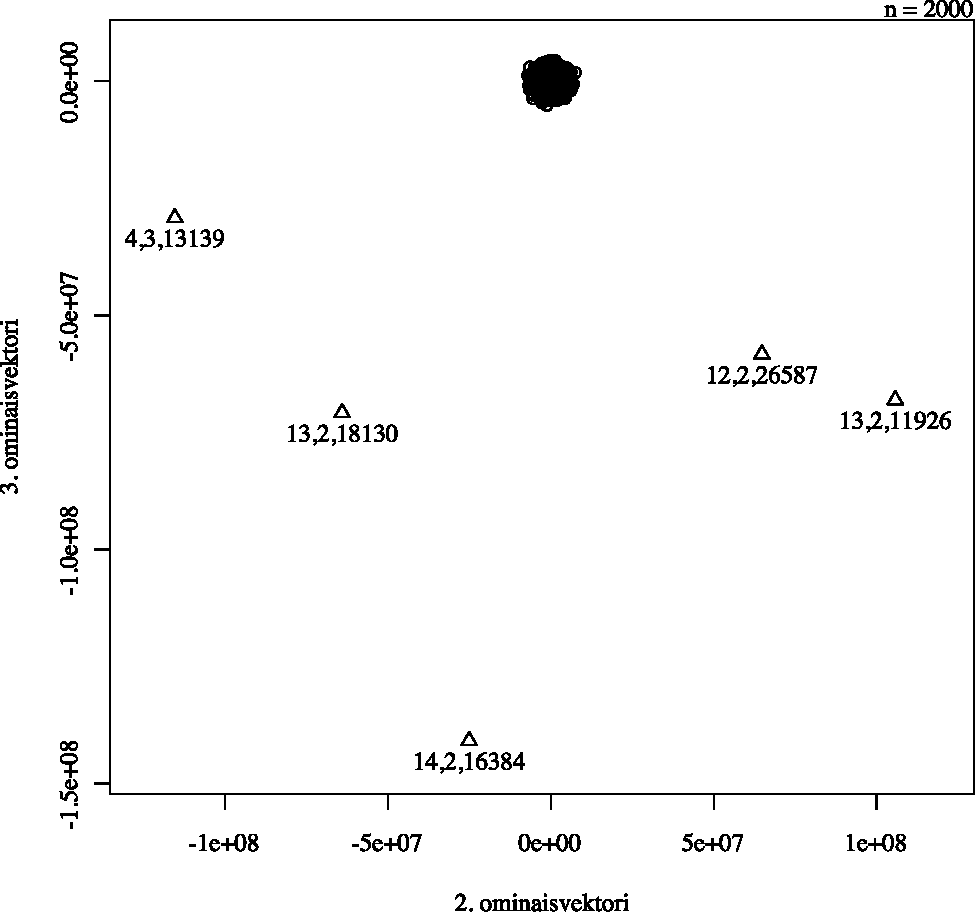
\includegraphics[width=10cm]{pics/diffuusiokuvat/service_1.pdf}
\caption{Resurssin 1 täristetty diffuusiokartta.}
\label{diffuusio_1}
\end{figure}

\begin{figure}[p]
\centering
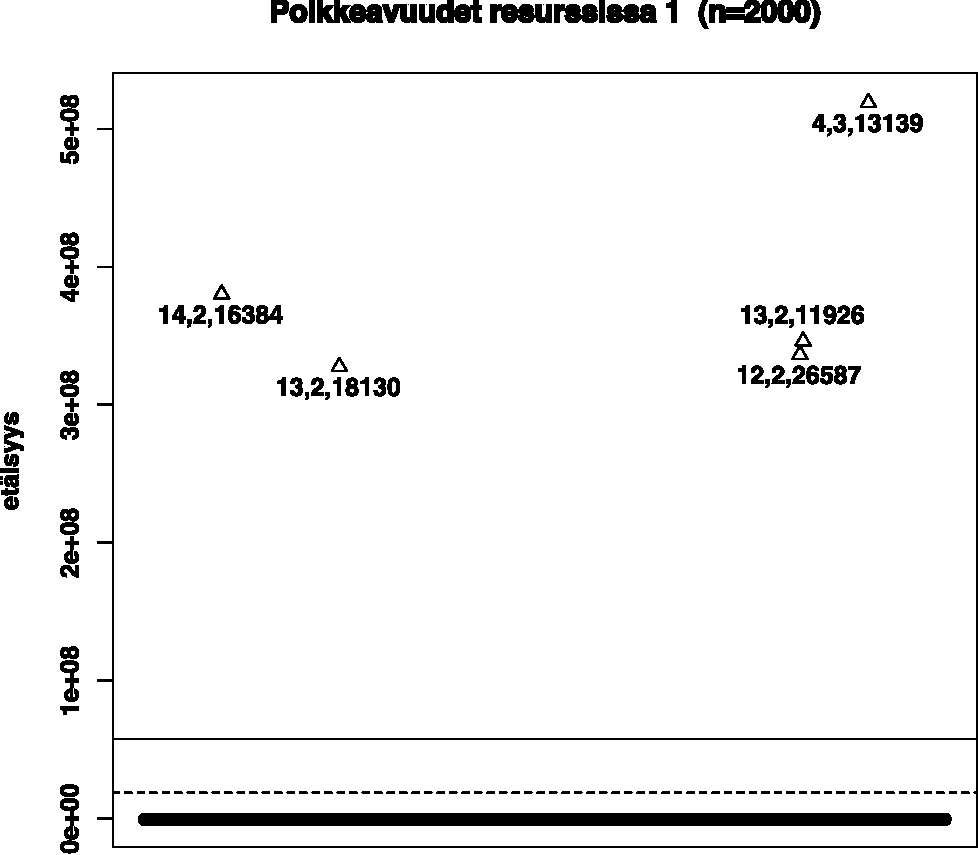
\includegraphics[width=10cm]{pics/tiheyskuvat/service_1.pdf}
\caption{Resurssin 1 poikkeavuuskartta.}
\label{service_1}
\end{figure}

\begin{figure}[p]
\centering
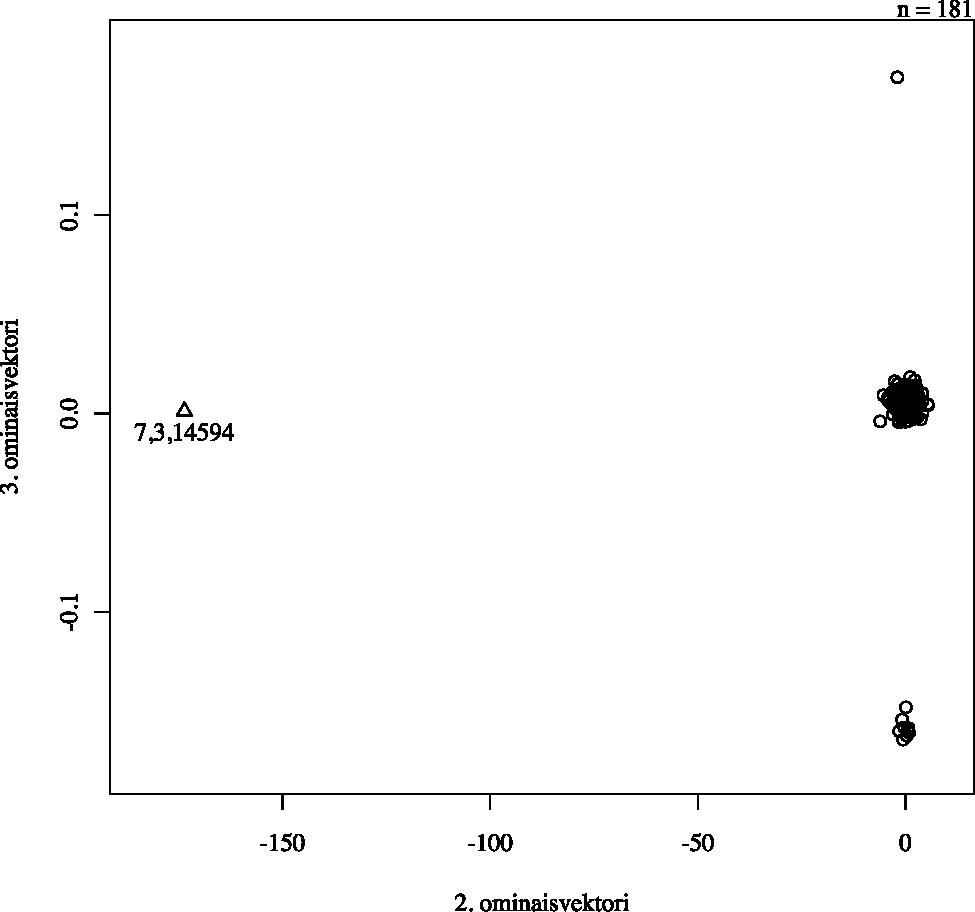
\includegraphics[width=10cm]{pics/diffuusiokuvat/service_18.pdf}
\caption{Resurssin 18 täristetty diffuusiokartta.}
\label{diffuusio_18}
\end{figure}

\begin{figure}[p]
\centering
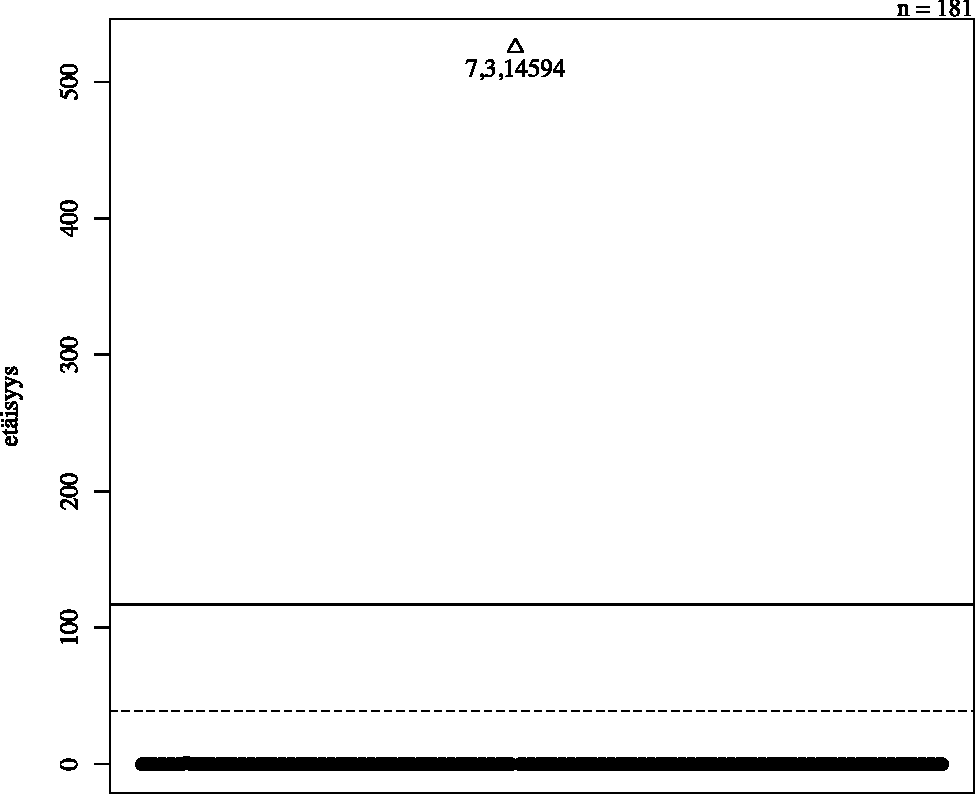
\includegraphics[width=10cm]{pics/tiheyskuvat/service_18.pdf}
\caption{Resurssin 18 poikkeavuuskartta.}
\label{service_18}
\end{figure}

\begin{figure}[p]
\centering
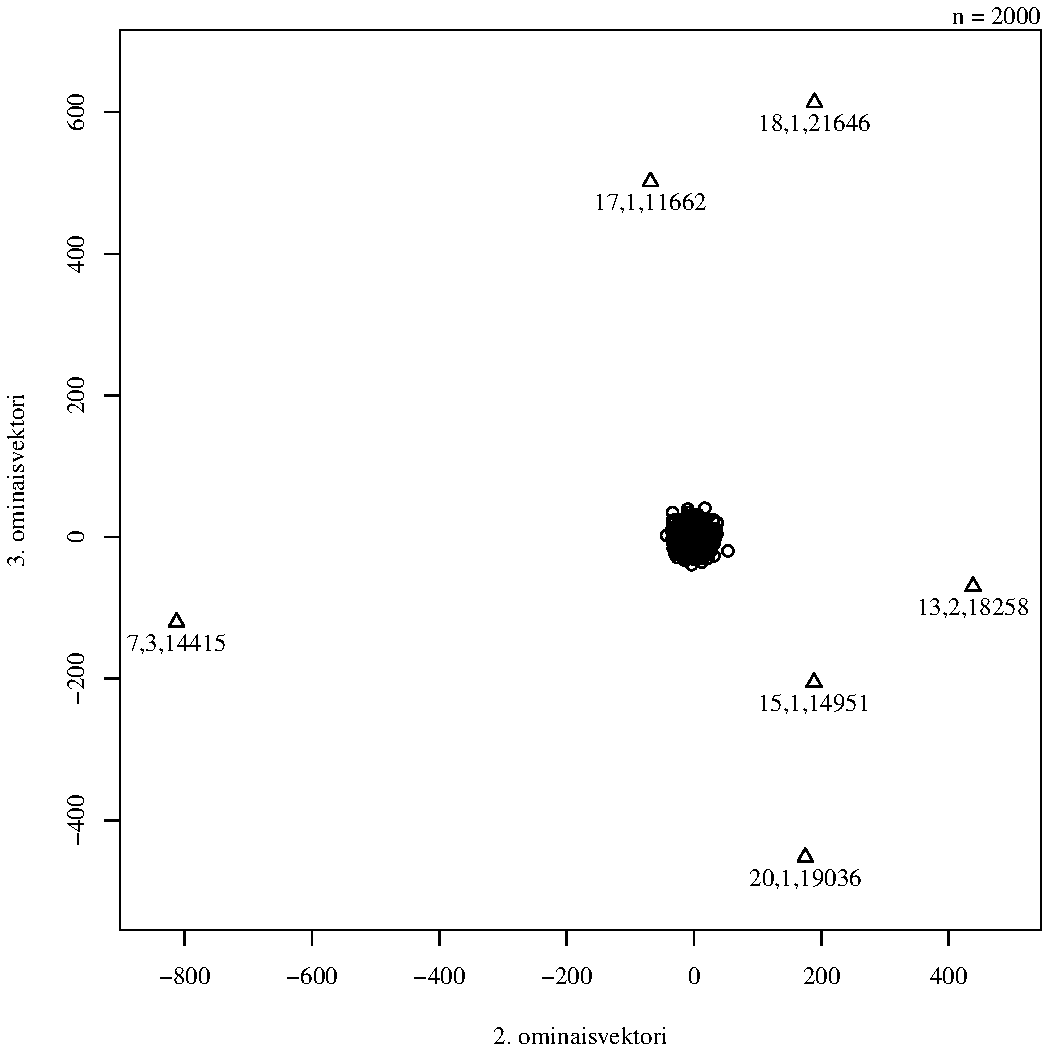
\includegraphics[width=10cm]{pics/diffuusiokuvat/service_337.pdf}
\caption{Resurssin 337 täristetty diffuusiokartta.}
\label{diffuusio_337}
\end{figure}

\begin{figure}[p]
\centering
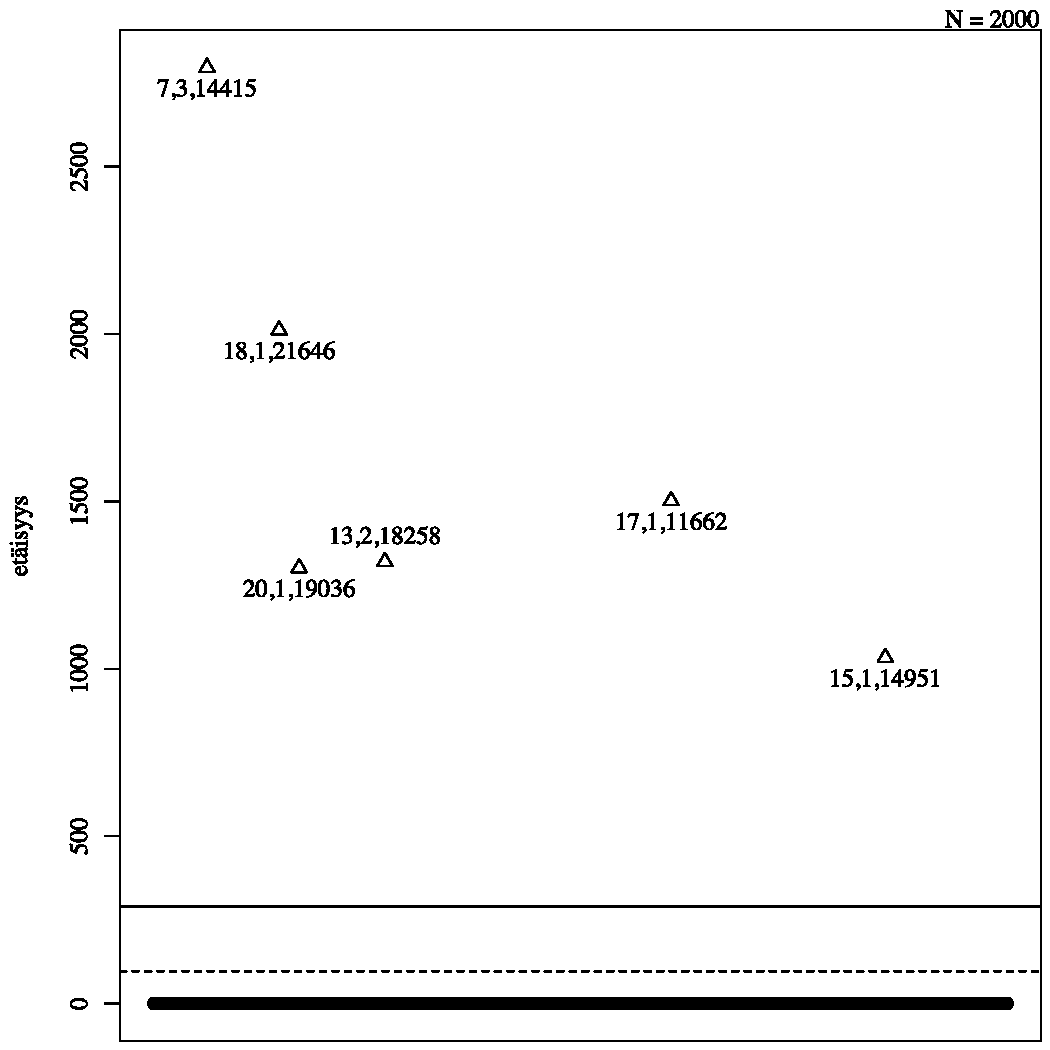
\includegraphics[width=10cm]{pics/tiheyskuvat/service_337.pdf}
\caption{Resurssin 337 poikkeavuuskartta.}
\label{service_337}
\end{figure}

\begin{figure}[p]
\centering
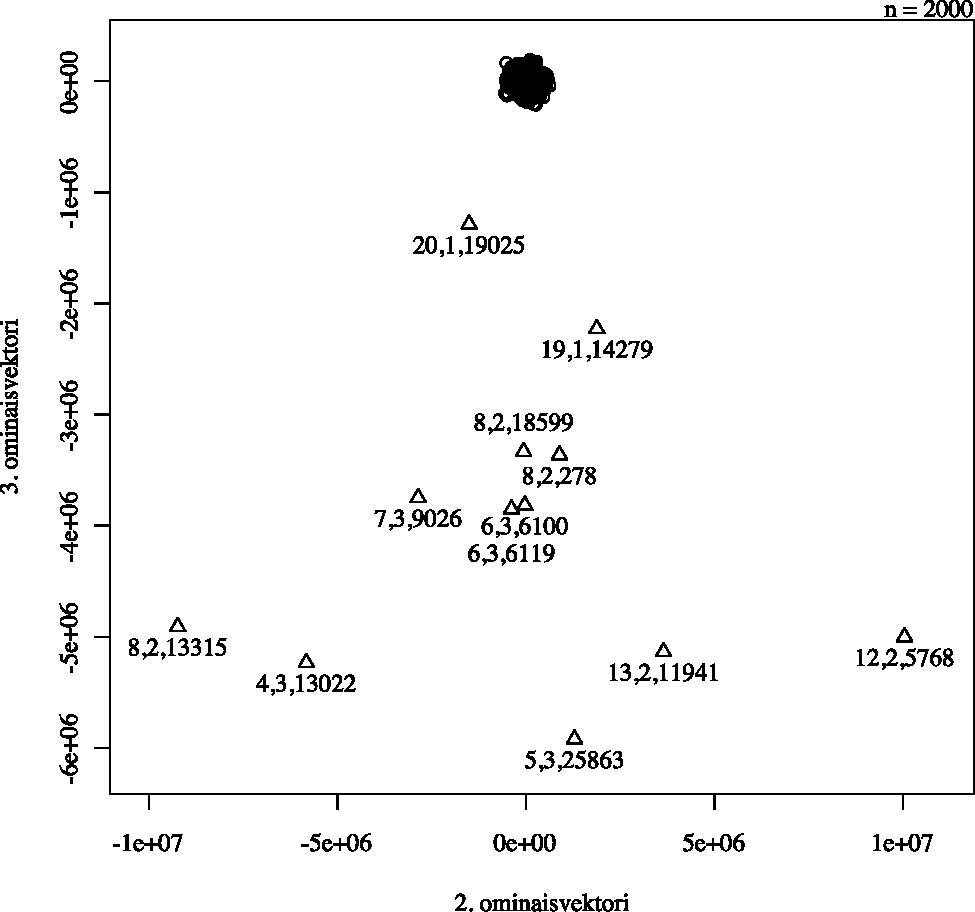
\includegraphics[width=10cm]{pics/diffuusiokuvat/service_721.pdf}
\caption{Resurssin 721 täristetty diffuusiokartta.}
\label{diffuusio_721}
\end{figure}

\begin{figure}[p]
\centering
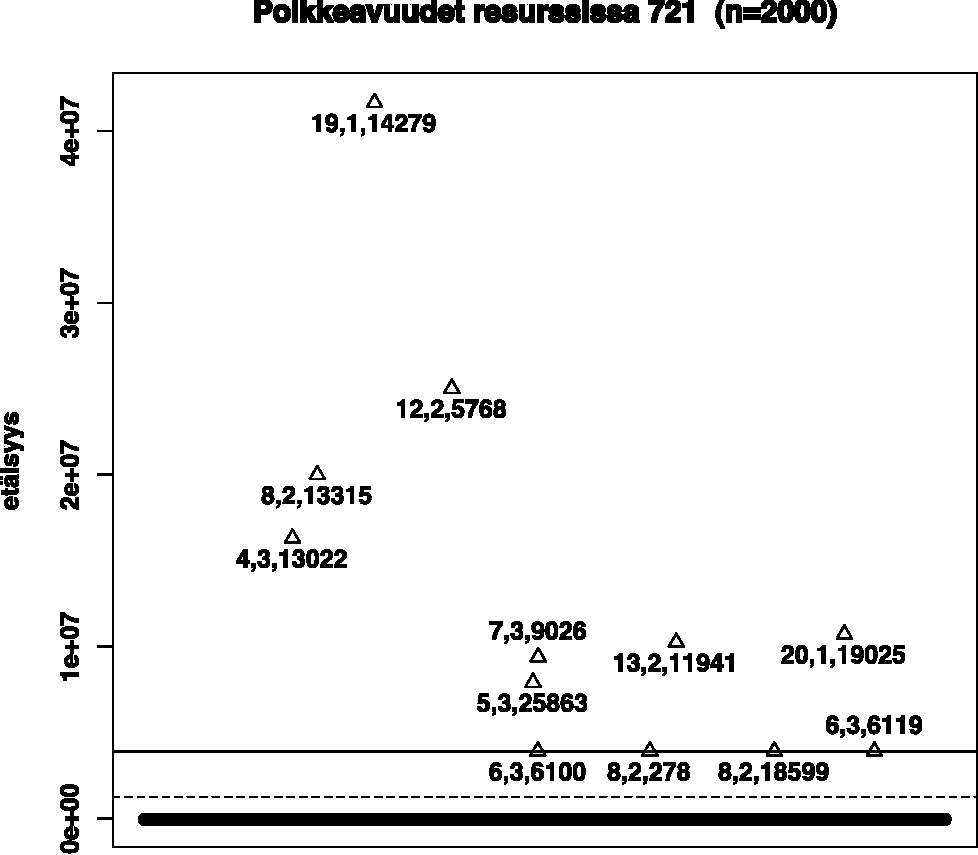
\includegraphics[width=10cm]{pics/tiheyskuvat/service_721.pdf}
\caption{Resurssin 721 poikkeavuuskartta.}
\label{service_721}
\end{figure}

\begin{figure}[p]
\centering
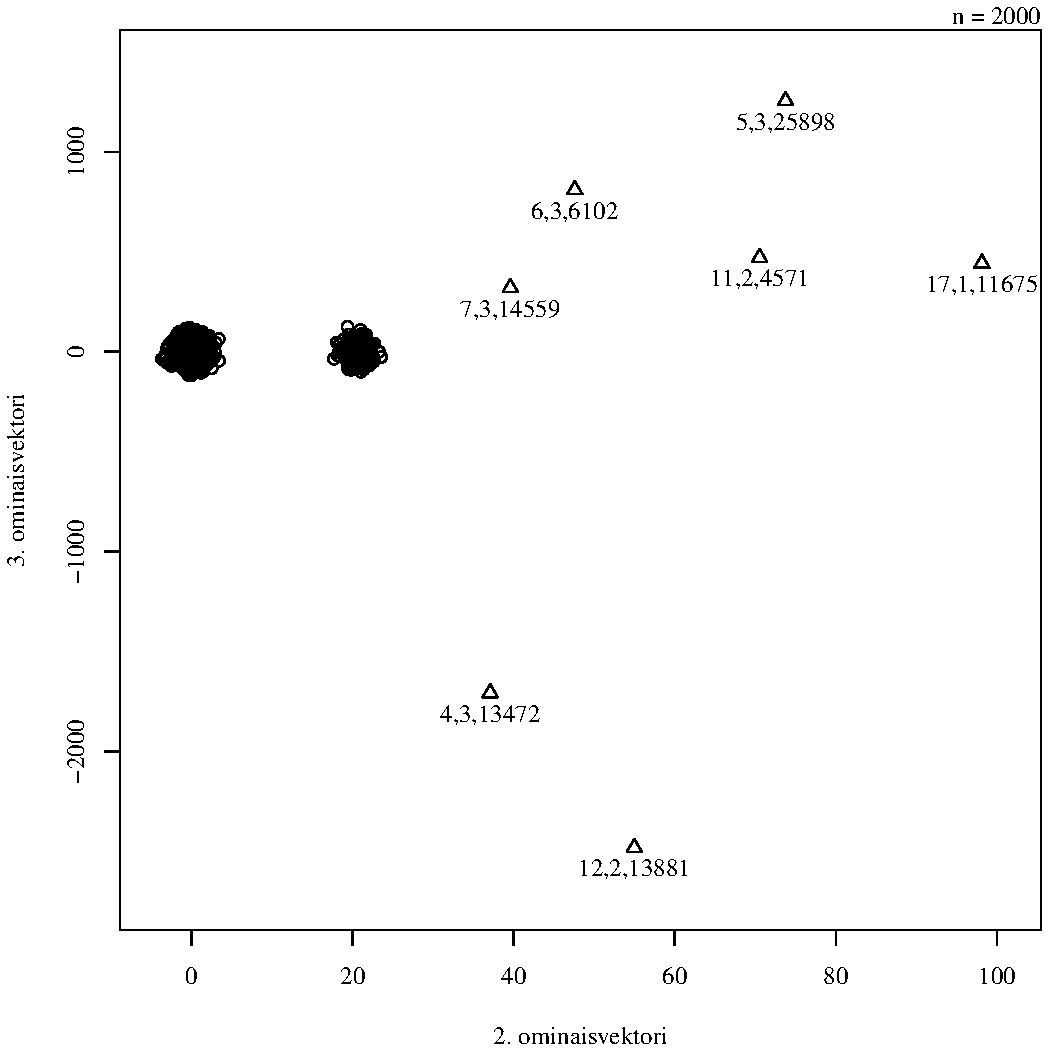
\includegraphics[width=10cm]{pics/diffuusiokuvat/service_723.pdf}
\caption{Resurssin 723 täristetty diffuusiokartta.}
\label{diffuusio_723}
\end{figure}

\begin{figure}[p]
\centering
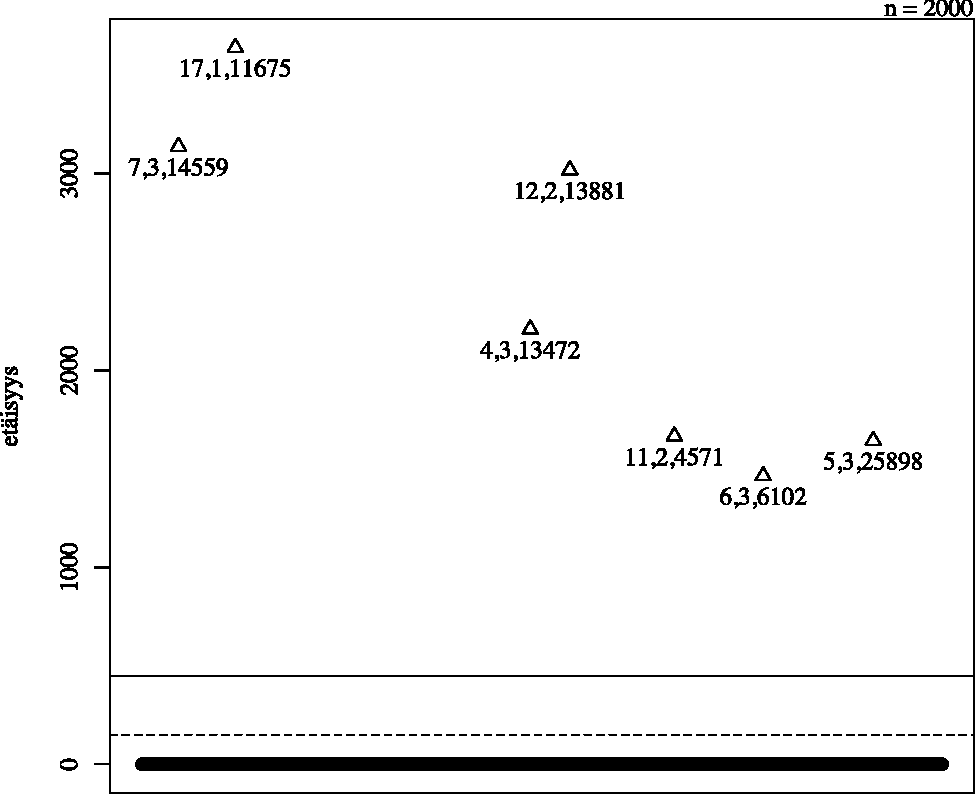
\includegraphics[width=10cm]{pics/tiheyskuvat/service_723.pdf}
\caption{Resurssin 723 poikkeavuuskartta.}
\label{service_723}
\end{figure}

\begin{figure}[p]
\centering
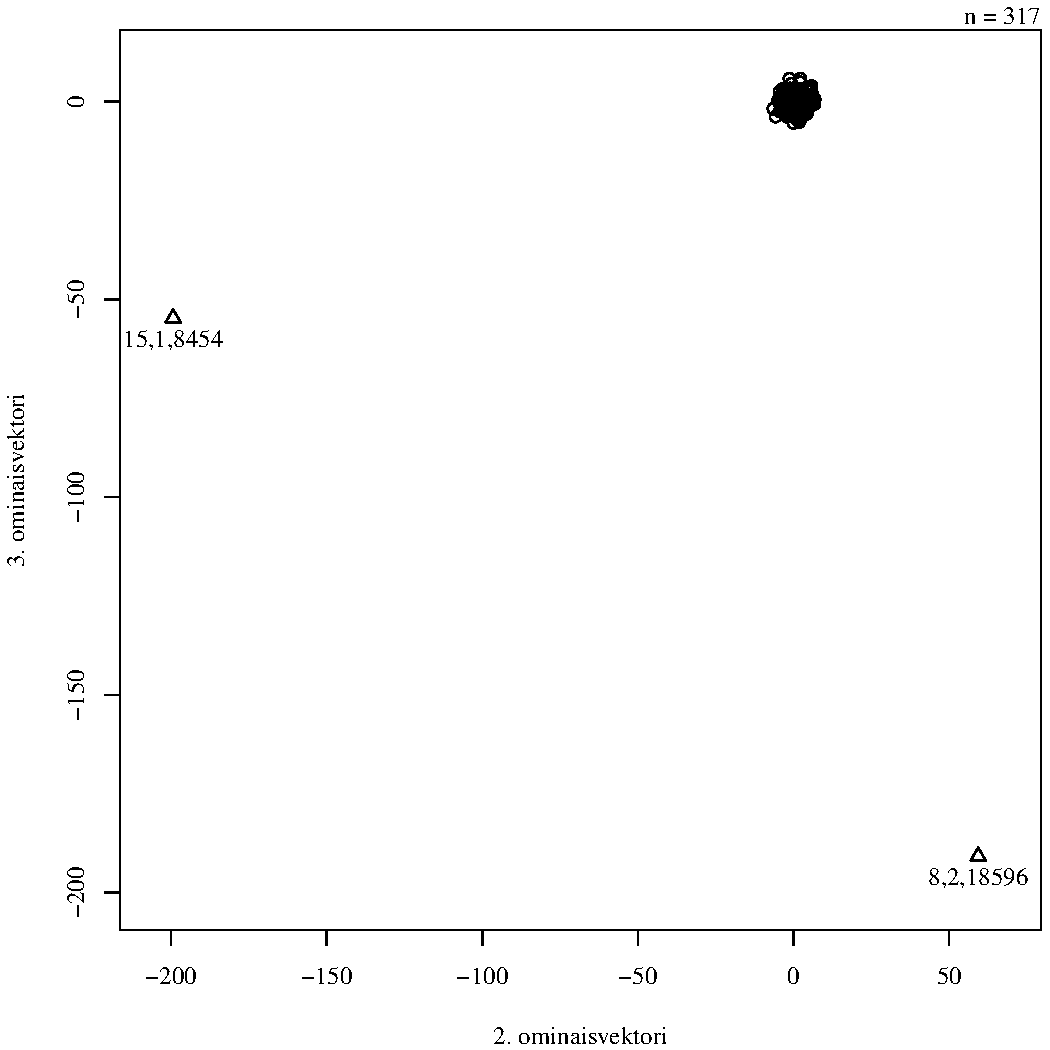
\includegraphics[width=10cm]{pics/diffuusiokuvat/service_882.pdf}
\caption{Resurssin 882 täristetty diffuusiokartta.}
\label{diffuusio_882}
\end{figure}

\begin{figure}[p]
\centering
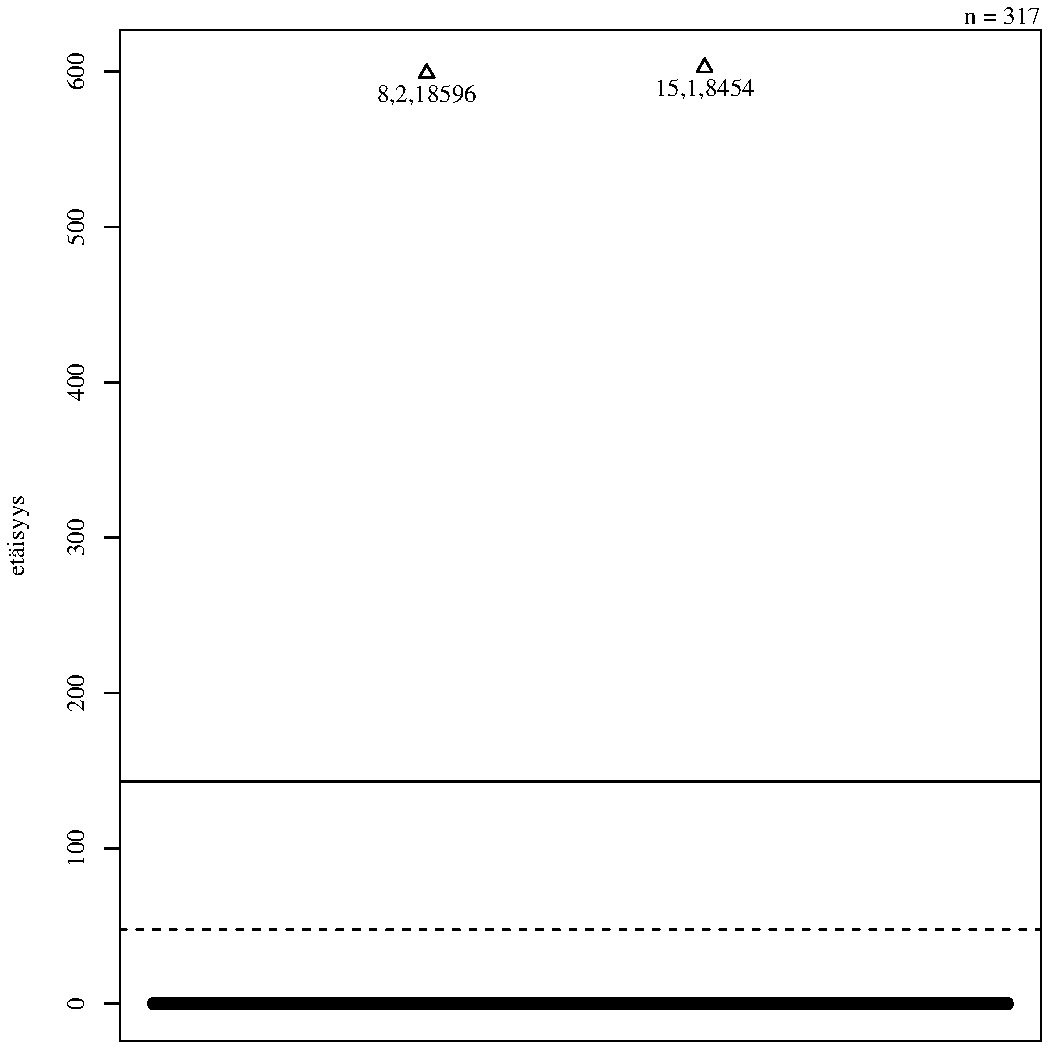
\includegraphics[width=10cm]{pics/tiheyskuvat/service_882.pdf}
\caption{Resurssin 882 poikkeavuuskartta.}
\label{service_882}
\end{figure}

\pagebreak

\section{Johtopäätöksiä ja kehitysideoita}

Analyysissä tuli hyvin esille se, että suurin osa liikenteestä oli
hyvin samankaltaista. Tutkittavan materiaalin osalta tätä osattiin
odottaa, mutta erilaisten pyyntöjen pieni valikoima yllätti siitä
huolimatta. Ja vaikka kyseisestä otannasta ei varsinaisia
tietoturvahyökkäyksiä löydetty, olimme tyytyväisiä saatuihin
tuloksiin. Tulokset osoittivat selkeästi sen, että esikäsittelijä
toimii halutulla tavalla ja valittujen menetelmien avulla poikkeavat
pyynnöt pystytään paikallistamaan.

Valtavasta tietomassasta johtuen aineistosta pystyttiin käytettävissä
olleen ajan puitteissa analysoimaan vain murto-osa. On siksi täysin
mahdollista, että palveluun kohdistuneita tietomurtoyrityksiä jäi
havaitsematta. Analysoidut palvelut saattoivat myös olla sellaisia,
joihin ei kohdistu kiinnostusta hyökkääjien keskuudessa.

Vaikka tässä työssä diffuusiokuvausten laskentaan käytetyn algoritmin
kompleksisuus rajoitti jonkin verran analyysin tekemistä, ei tämä
käytännön toteutuksessa muodostune kuitenkaan
ongelmaksi. Reaaliaikaisessa toteutuksessa järjestelmälle voidaan
opettaa etukäteen normaali käyttäytyminen diffuusiokuvauksen avulla,
jonka jälkeen uusien pisteiden paikka vertailujoukossa lasketaan
yksitellen. Tällöin algoritmin aikavaativuus riippuu ainoastaan
opetusjakson koosta, eikä analysoitavien pisteiden määrästä. Uudet
pisteet voidaan projisoida diffuusioavaruuteen esimerkiksi Nyströmin
laajennuksen avulla, jota ei tähän työhön enää otettu
mukaan.

Opetusjakson tarkempi määrittely tarjoaisi analyysin kannalta
hyödyllisempää tietoa. Jatkokehityksessä seuraava askel olisi
analysoida tarkemmin valikoitua materiaalia. Tämä voisi tarkoittaa
esimerkiksi lokin analysointia sellaiselta ajanhetkeltä, jolloin tiedetään
tietomurtoyritysten tapahtuneen. Tätä liikennettä voitaisiin verrata
normaalitilanteeseen ja näin tunnistaa piirteitä, jotka erottavat
poikkeavan liikenteen normaalista.  Tällaisen aineiston käyttö
tarjoaisi erinomaiset puitteet testata tässä työssä käytettyjä
ratkaisuja.

Toinen kehityssuunta olisi kehittää esikäsittelymenetelmiä. Tämä voisi
tarkoittaa esimerkiksi sitä, että palvelinlokista kerättäisiin enemmän
piirteitä, joista voitaisiin muodostaa enemmän parametreja
diffuusiokuvasta varten. Tällaisia piirteitä olisi esimerkiksi
käyttäjän IP-osoite ja Web-selaimen tunnistetieto. IP-osoitteen
luokittelussa voitaisiin hyödyntää esimerkiksi tarjolla olevia
GeoIP-\-tietokantoja. Käyttäjän IP-osoitteesta voitaisiin näin
selvittää esimerkiksi palveluntarjoaja, jonka kautta kysely
tuli.

Käyttämämme esikäsittelijä ei myöskään hyödynnä kyselyiden ajallista
riippuvuutta eikä ryhmittele kyselyitä muuten kuin resurssien
perusteella. Esikäsittelijää voisi laajentaa siten, että se mittaisi
esimerkiksi samasta osoitteesta tulevien kyselyiden tiheyttä. Näin
olisi mahdollista tunnistaa nykyistä paremmin purskeista liikennettä,
joka usein liittyy palvelunestohyökkäyksiin.

Poikkeavuuksien tunnistamisessa voitaisiin käyttää Apache-lokin
rinnalla myös muita tietolähteitä. Tällaisia olisivat esimerkiksi
palvelinten muistinkulutus ja prosessorikuormitus. Lisäksi
Web-palvelimen toiminnasta voisi kerätä myös sellaisia parametreja,
joita ei yleisesti kerätä lokeihin. Esimerkkinä kyselyihin vastaamiseen kulunut
aika ja resurssit. Tietoa voisi kerätä myös verkkokerrokselta,
jolloin voitaisiin havaita sellaiset hyökkäykset, joita ei ole
mahdollista tunnistaa sovelluskerroksella.

% TODO: Kuinka eri poikkeavuuskartat saisi "yhteismitallisiksi", eli
% voisi mitata koko palvelun poikkeavuuksia samalla kertaa.
